\section{Photodetector position}\label{sec:mppcposition}
The location of each photodetector is determined using charge
generated in the photodectectors by X-ray interactions corresponding
to a precisely placed source.  An outline of the detector is created
by X-ray events and fitted to determine the center position (fig
\ref{fig:xrayevents}). 

\begin{figure}[h]
  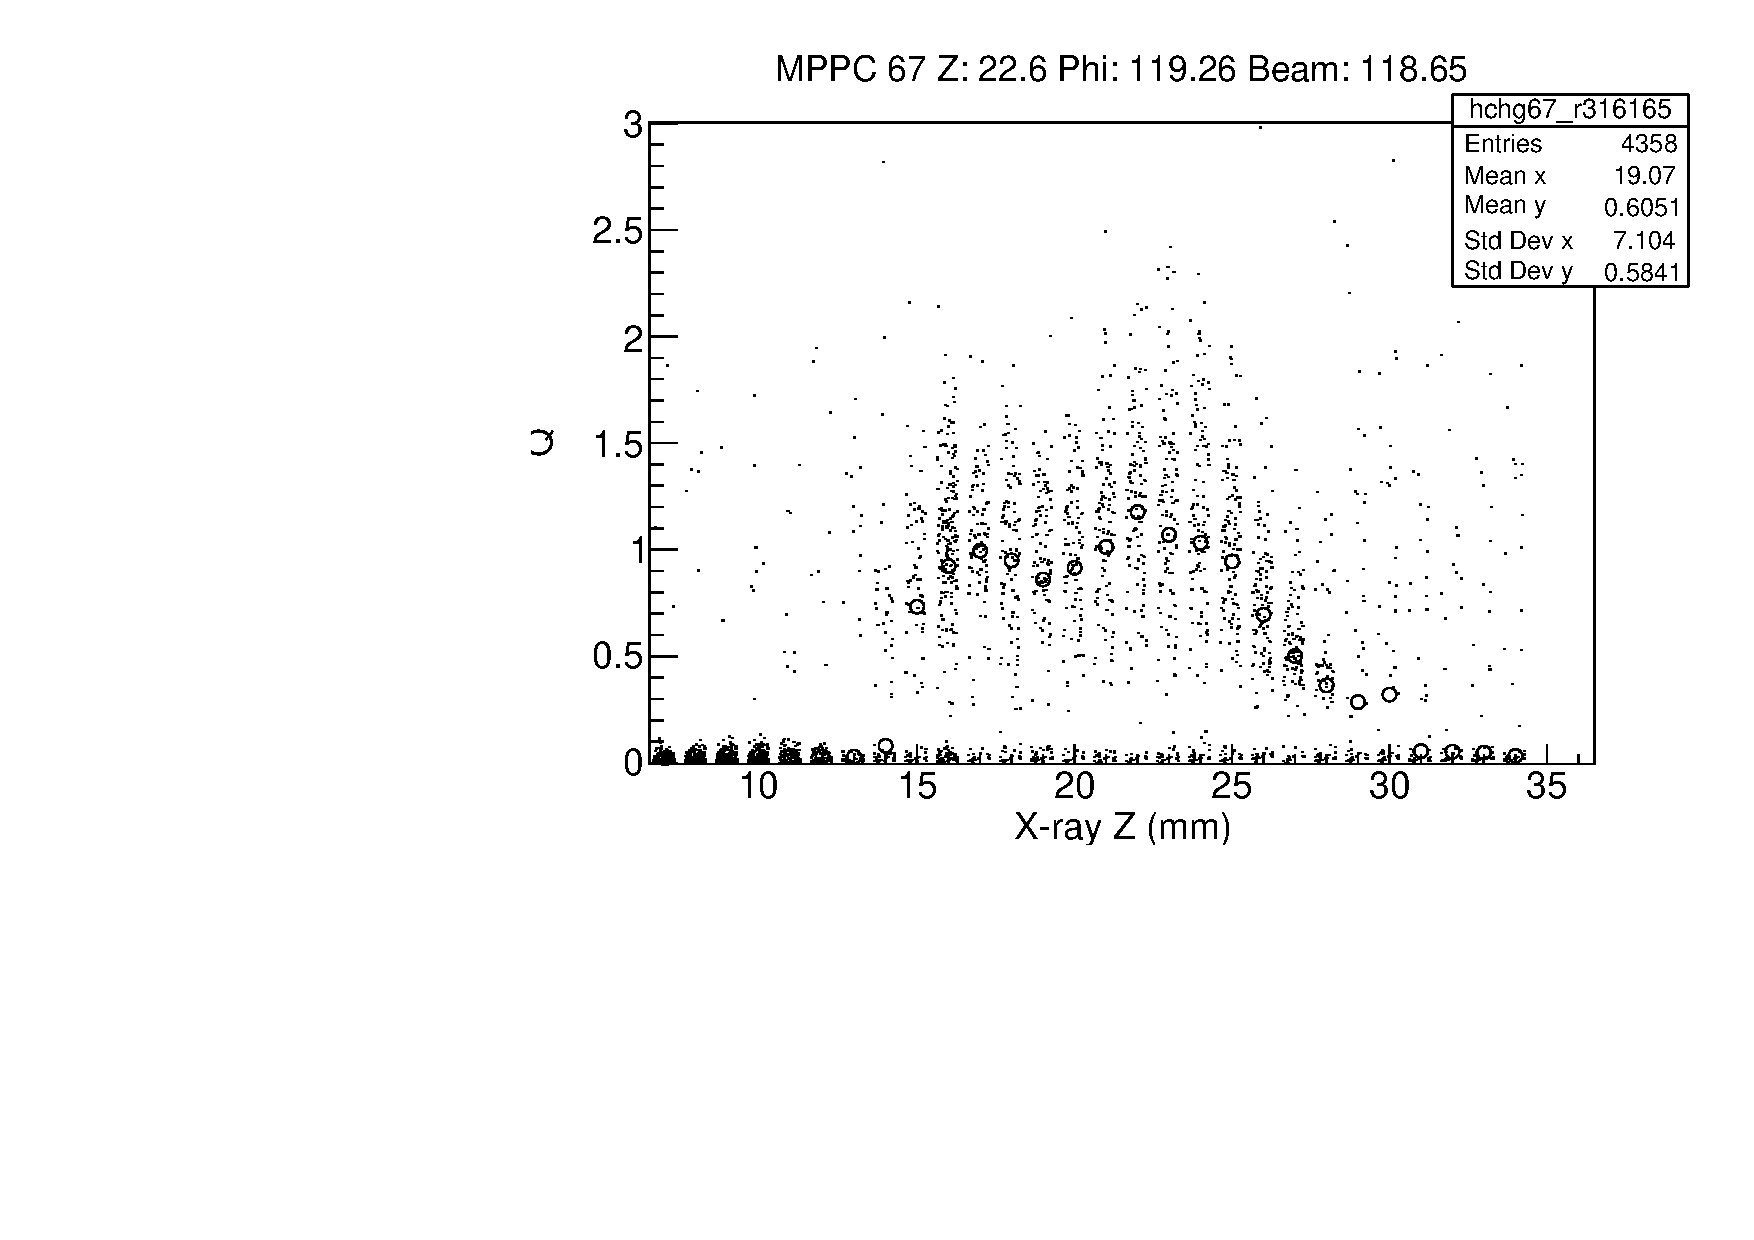
\includegraphics[width=4cm]{plots/2018/hcharge67_z}
  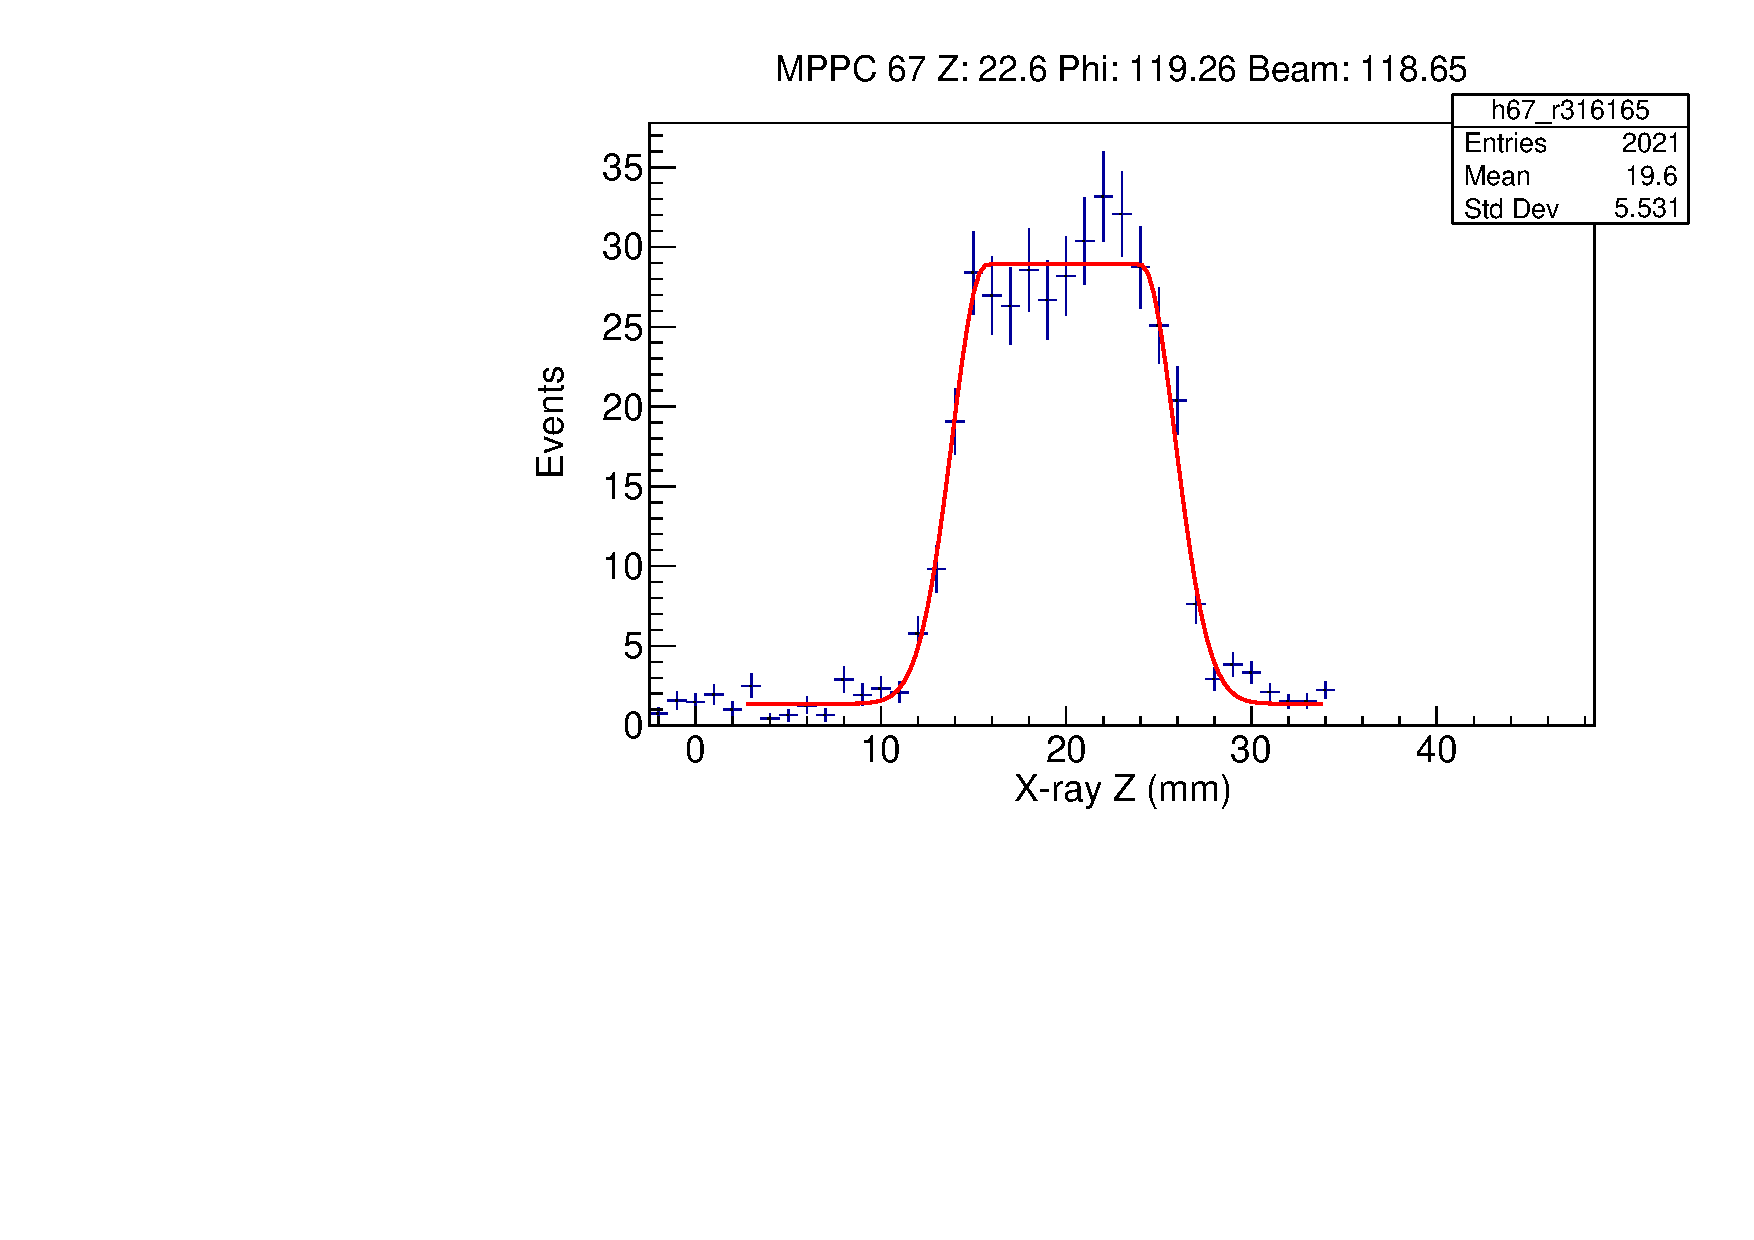
\includegraphics[width=4cm]{plots/2018/mppc_fit}
  \caption{Charge recorded in a single photodetector as a function of X-ray Z coordinate 
  (left) and 
    the calculated event rate (right).}
  \label{fig:xrayevents}
\end{figure}  

To isolate signal events, a trigger threshold on cumulative charge 
in the region of scanned photodetectors is applied with background 
subtraction to exclude coherent electronic noise. Additionally, 
an offline selection criteria matching X-ray energy pattern are applied
requiring large absolute charge in the channel 
($>0.6$~pC), a summed trigger waveform with peak-time in the correct timing window ($-0.7\mu$s,$-0.5\mu$s), and simultaneously a small average deposition 
in the background channels ($<0.2$~pC).

The X-ray event rate as a function of X-ray position ($z/\phi$) is
fitted with the following peicewise continuous function,\\
\begin{math}\label{eqn:mppcfitfcn}
f(z) = 
\begin{cases}
   b+s\cdot 
Exp\left[-\frac{(z - \, (\mu_m - w/2)\,)^2}{\sigma_m^2}\right] & z <
\mu_m-w/2  \vspace{3mm} \\
   b+s\cdot 
Exp\left[-\frac{(z - \, (\mu_m + w/2)\, )^2}{\sigma_m^2}\right] & z >
\mu_m+w/2    \vspace{3mm} \\
   b+s                                         & \mu_m - w/2 < z < \\
                                               & \mu_m + w/2    \\
\end{cases}
\end{math}

\noindent where, $w$ and $\mu_m$ are the width and center position of
the photodetector, $\sigma_m$ gaussian width of the edges, and $s,\,b$
are the signal and background event rates. A sample of well fitted
photodectector locations is used for  subsequent analysis.

The X-ray scans together with the fitted radial coordinate (described
in the next section) provide a 3D
location of each scanned photodetector  with high precision
($\sigma_{|\vec{x}|}<0.5$~mm).  These measurements are compared to a set of
nominal positions in the designed detector in order to reveal changes due to
manufacturing and installation.  Secondly, the two X-ray  measurements are
fitted to find global offsets in the absolute positions which could be
introduced due to the movement of the calorimeter or thermal cycling of LXe
scintillator conducted between the two scans.

The nominal positions of the photodetectors ($Z_{MPPC}$,
$\phi_{MPPC}$) are in a regular grid along a cylindrical surface with
constant radius, and its central axis aligned with the Z axis of the
MEG coordinate system.  From direct measurements in FARO and X-ray
surveys (described in the next section), we have shown  that the
radial coordinate of the photodetectors is not perfectly uniform.  We
find that the calorimeter can be divided into four separate regions
formed by the cfrp plates. Within each plate there is rotation of the
photodetectors about the radial axis which causes $\phi$ dependent
variation in the Z coordinate, and corresponding and equal Z dependent
variation in the $\phi$ coordinate of the MPPC measured by the X-ray
scan (figures \ref{fig:rotation1}, \ref{fig:rotation2}). The deviation of the measured from
the nominal in Z and $\phi$ coordinates is fitted independently on
mutiple subsets of photodetectors within each cfrp plate. The results
(table \ref{tab:rotation}) show the mean slope due to the rotation
varies between 2-5~mrad  or 1-4~mm displacement of the photodetector
over the entire calorimeter.
A consistently higher slope of  $d\phi/dZ$ compared to $dZ/d\phi$
indicates a 1~mrad deviation in the construction of the cfrp plate
from a perfectly 
rectilinear assembly board in the z-$\phi$ plane.  The figures and the
table show calculations using 2017 data, the results from the smaller
2018 data are found to be identical but not used. 

\begin{table}
\begin{tabular}{ccc}
   & $dZ/d\phi_{MPPC}$ & $d\phi/dZ_{MPPC}$ \\
\hline 
cfrp 1 & -0.0025 & 0.0033 \\
cfrp 2 & -0.0032 & 0.0040 \\
cfrp 3 & -0.0033 & 0.0045 \\
cfrp 4 & -0.0050 & 0.0058 \\
\end{tabular}
\caption{Average slopes (mm/mm) of deviation between X-ray and nominal MPPC positions
$dZ, d\phi$ with respect to the other coordinate, shown for each 
cfrp plate.}
\label{tab:rotation}
\end{table}

\begin{figure}
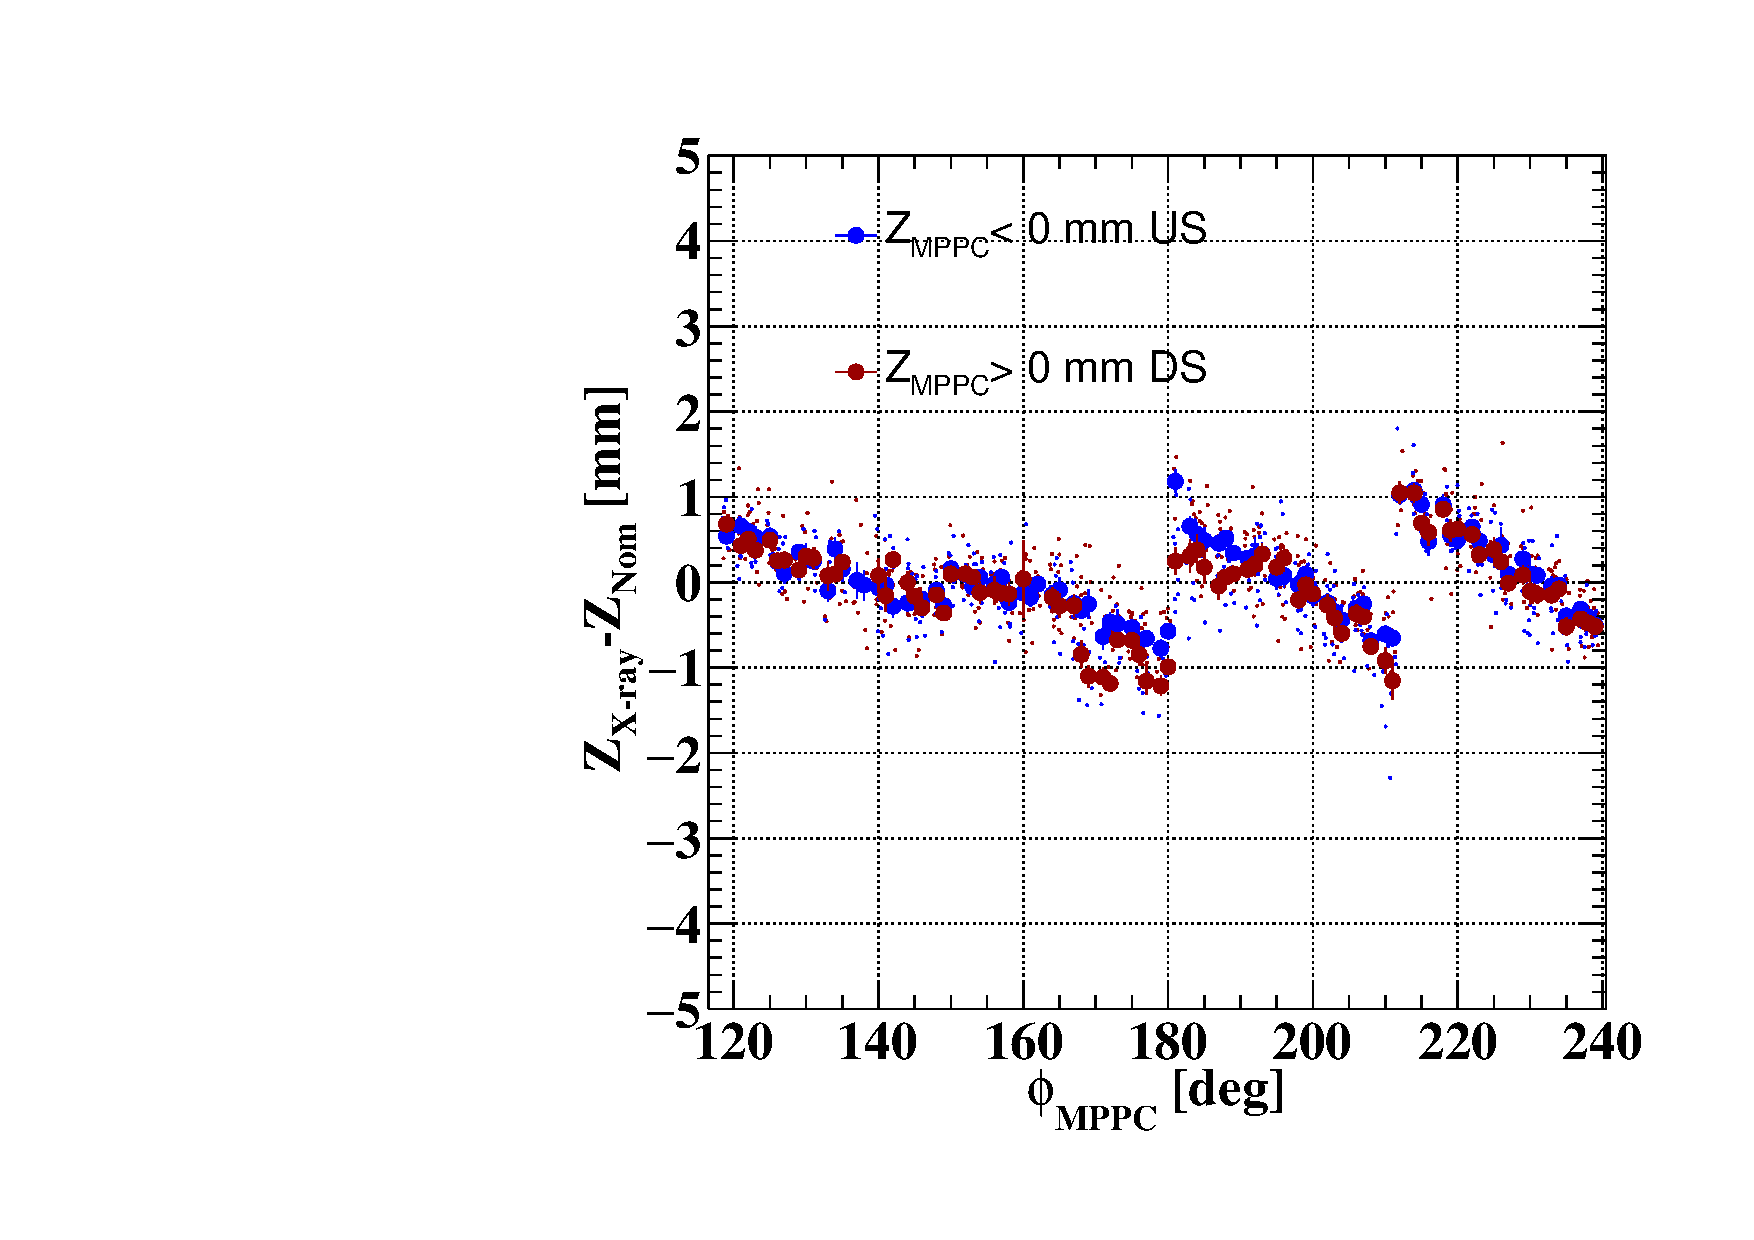
\includegraphics[width=4cm]{plots/dz_boardrotation.pdf}
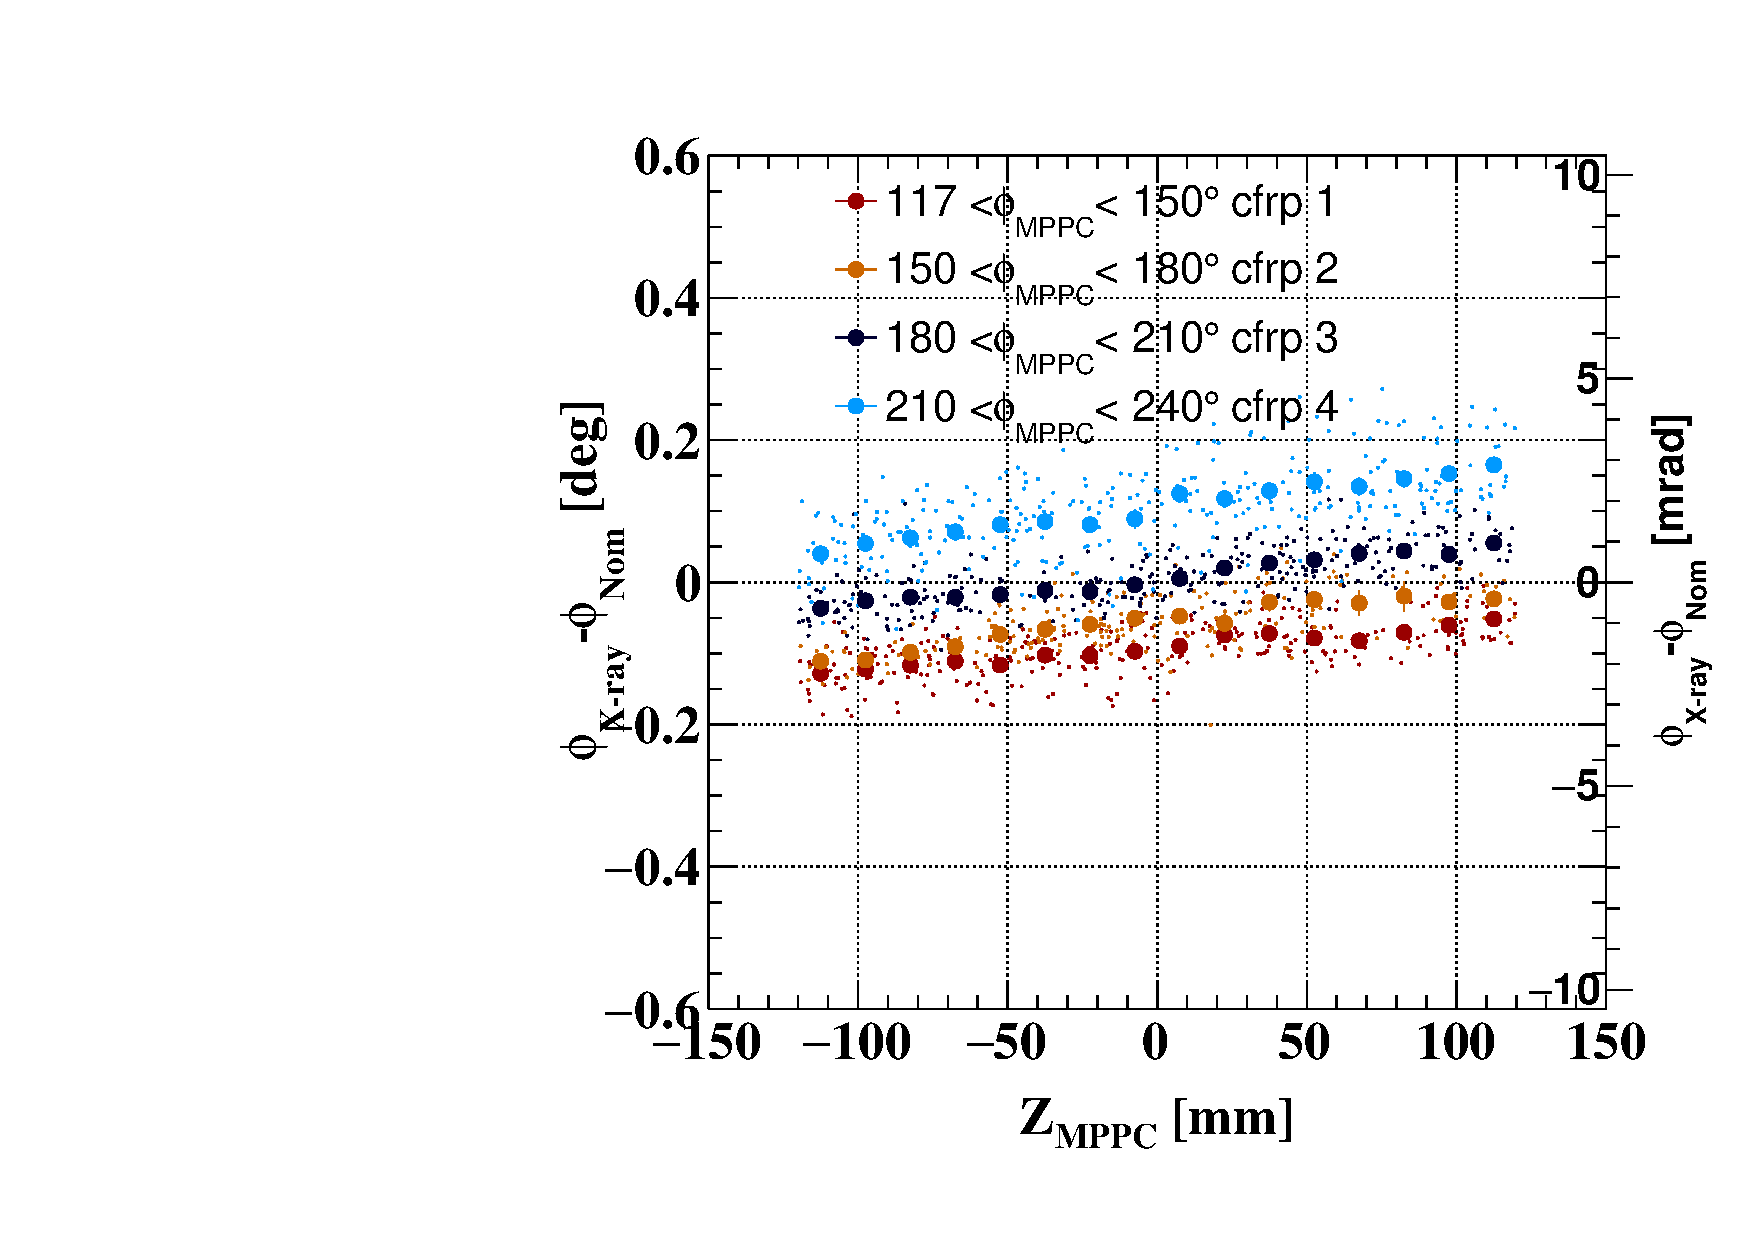
\includegraphics[width=4cm]{plots/dphi_boardrotation.pdf}\\
\caption{[add cfrp boundary]
Difference between the X-ray measured and nominal MPPC positions
overlayed with the profile histogram (scatter plots).
US and DS PCB half-strips and cfrp plates are shown separately.
Both Z and $\phi$ measurements have global offsets with respect to the 
nominal which are corrected in the plots.
}
\label{fig:rotation1}
\end{figure}

\begin{figure}
\begin{center}
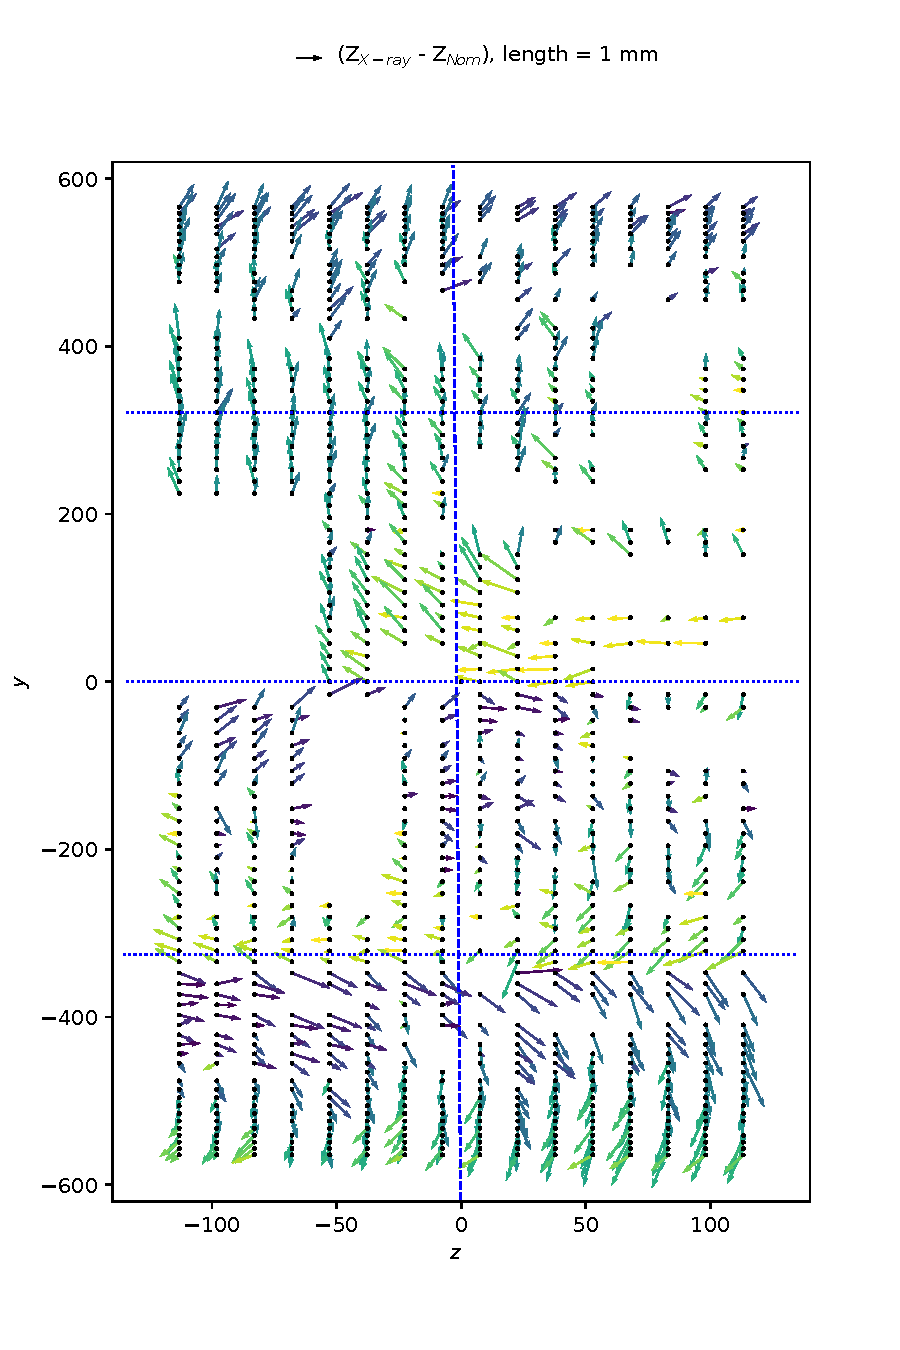
\includegraphics[width=6cm]{plots/dzdy2017_rx_test.pdf}
\caption{Arrow plot showing rotation of the MPPCs with respect to nominal
positions in the YZ plane; dotted horizontal lines show cfrp plate boundaries,
dashed vertical line at the center separates the PCB half-strips.
Both Z and $\phi$ measurements have global offsets with respect to the 
nominal which are corrected in the plots.
}
\label{fig:rotation2}
\end{center}
\end{figure}


The stability of the reconstructed position 
is verified by testing its dependence on 
the analysis procedure in two ways. 
First, the X-ray selection is performed using another independent criteria
and the fitting procedure is repeated.
Second, a different fitting function with higher-order Gaussian is
used. The pattern of X-ray event rates in each photodetector is fitted with
the function

\begin{equation} \label{eqn:supergauss}
    f(z)=b+s\cdot
Exp\left[-\left(\frac{z-\mu_{m}}{\sigma_{w}}\right)^{8}\right],
\end{equation}

where $b,s$ are the signal and background event rates. The 
flat-top of the function is centered at $\mu_m$,
and $\sigma_w$ determines the size  of
flat-top as well as the gaussian width of fall-off
on both sides. 
The results show new reconstructed positions consistent with the initial
calculation with mean 0.07~mm (0.2 mrad) and standard deviation
0.3~mm (0.45 mrad).

